% !TEX root = ../thesis-example.tex
%
\externaldocument{content/survey}
\externaldocument{content/registration}
\externaldocument{content/viewpoint}
\externaldocument{content/ExGOER}
\externaldocument{content/omnipresent}
\chapter{Introduction}
\label{sec:intro}

\cleanchapterquote{There is a difference between knowing the path and walking the path.}{Morpheus}{The Matrix}
%\cleanchapterquote{Learning is more effective when it is an active rather than a passive process.}{Kurt Lewin}{}
\begin{figure}[b!]
	\centering
	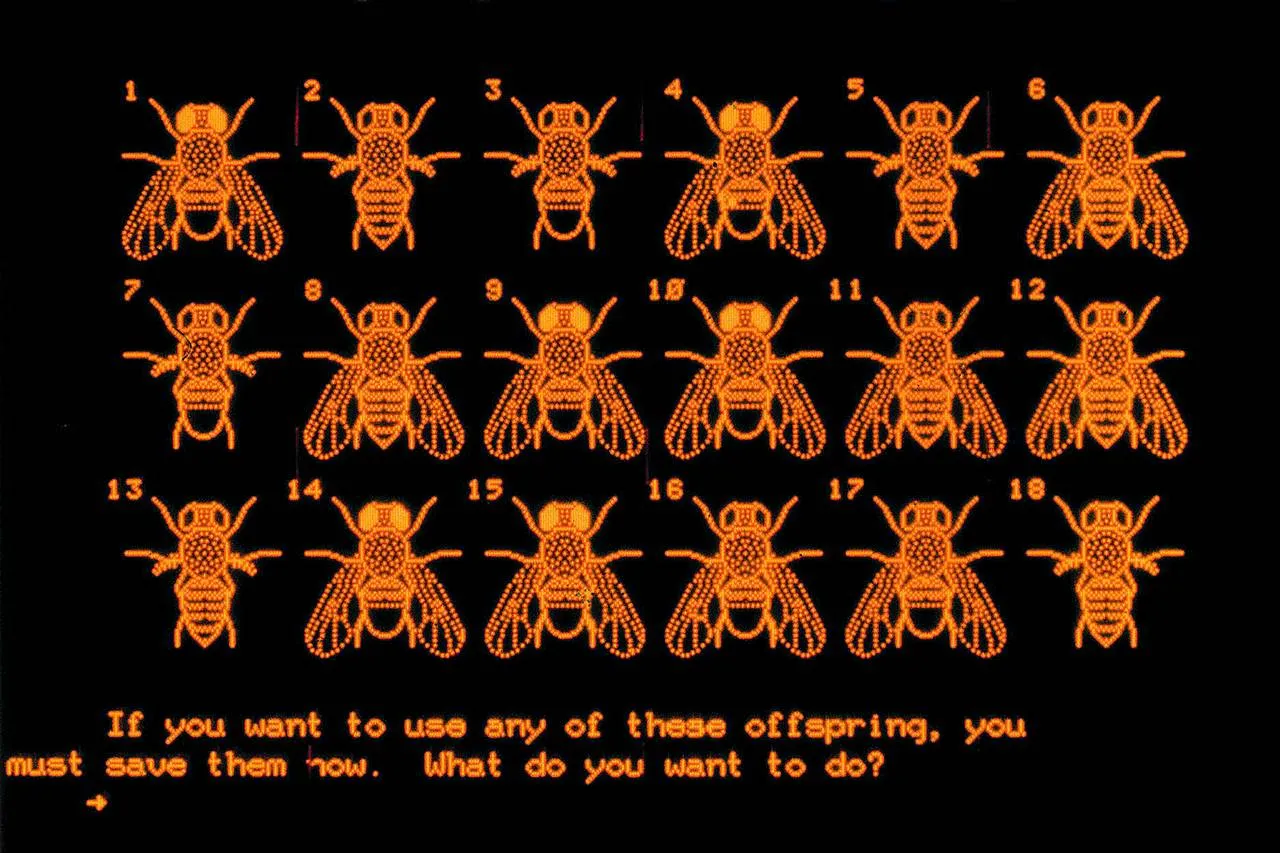
\includegraphics[width=\linewidth]{pictures/plato.png}
	\captionsetup{labelfont=bf,textfont=it}
	\caption[Educational visualizations on the \acrshort{plato} system. Taken from \cite{lapsley2017review}]{One of the earliest educational visualizations on the \acrshort{plato} IV learning system. Image by Paul Tenczar \cite{lapsley2017review} \label{fig:plato}}
\end{figure}

Since the earliest days of computers, they have been leveraged as a tool for teaching.
The use in universities, which serve as both --- research and education facilities --- seems to have established computers being used in both areas.
One of the earliest computer teaching systems was developed in 1959 with the \acrlong{plato} --- short \acrshort{plato} --- at the University of Illinois \cite{cope2023history}.
The early emergence of educational technology suggests the importance of developing engaging learning tools.
Even in the earliest iterations of the \acrshort{plato} system, visual learning aids were applied as can be seen in \autoref{fig:plato}.
Schematics and graphs helped students to approach a subject from different angles.
Today, the importance of visualization in education is well established.
Computer-based visualizations are said to increase motivation and engagement of learners \cite{vavra2011visualization}.
In addition to visualization, interaction plays an important role in education \cite{firat2018towards}.
Kolb described interaction in 1984 \cite{kolb:1984:experiential} as a key aspect to creating experiences, which he found critical to establish learning (see also \autoref{sec:experiential}).
To leverage both these concepts to the fullest, suitable technologies have to be considered carefully.

The reality-virtuality continuum as defined by Milgram et al. \cite{milgram1994arc} represents a spectrum of environments ranging from real-world to entirely virtual, including various technologies summarized under the collective term \acrfull{xr} like Augmented (\acrshort{ar}), Virtual (\acrshort{vr}), Mixed Reality (\acrshort{mr}) and many more.
In recent years, the literature regarding \acrshort{ar} and \acrshort{vr} technologies in education has increased drastically \cite{alansi2023analyzing}.
These technologies have become increasingly more accessible and accepted.
However, the development, acquirement and application can still be more extensive than conventional technologies.
Therefore, web-based learning applications and dedicated learning programs still have their place depending on the use case.
This thesis will introduce a selection of interactive learning approaches, which represent different points on the reality-virtuality continuum. 

Located in the far virtual end of the continuum, \autoref{chap:ExGoer} presents a novel educational framework for \Acrfull{cg}.
It involves interactive learning applications as well as corresponding slides and quizzes.
This chapter provides a broad scope, as the framework itself can be applied to various use cases.
At the same time, it was applied to \acrshort{cg} and some of the topics offer an insight into the foundations for \acrshort{xr}.
Narrowing the scope, \autoref{chap:visualCueSurvey} provides a literature overview of visual feedback for motor skill learning in \acrshort{mr}.
Approaches covering a broad range of the reality-virtuality continuum were surveyed.
The publications were analyzed for specific visual cues and classified according to their visual cues, \acrshort{mr} technologies and more.
Venturing into one of the more prevalent visual cues --- superimposed human avatars, \autoref{chap:registration} examines the registration of superimposed avatars to provide a good foundation for motor feedback.
Drawing from this foundation, \autoref{chap:viewpoint} presents a novel method for viewpoint selection considering human poses and visual motor feedback in real time.
Lastly, \autoref{chap:omnipresent} introduces an innovative \acrshort{ar} system for visual motor feedback.
The system offers a comfortable method for receiving motor feedback that is independent of head position.
As a result, users are enabled to execute movements with a reduced risk of falsifying the exercise compared to conventional feedback systems, which could lead, in the worst case, to injuries.

All the above-mentioned chapters correspond to research questions, which will be discussed in detail in \autoref{chap:concepts}.


\begin{comment}
\section{Thesis Structure \label{sec:intro:structure}}
Firstly, \autoref{chap:ExGoer} introduces an interactive application framework for computer graphics education. The holistic modular approach allows for easy adaptation and creation of new open educational resources for teaching professionals.

Substantial parts of this thesis describe learning in the context of motor skills in mixed reality. To provide the fundamentals for this topic, \autoref{chap:visualCueSurvey} surveys existing literature for visual cues that are used in mixed reality to facilitate skill learning. From initially 131 works, 39 approaches were analyzed. Not only the visualization methods that helped learning were extracted, technologies, use cases and other details of the publications were revealed and interpreted as well.

Delving deeper into one of the more prevalent visual cues for learning motor skills --- superimposed human skeletal avatars --- \autoref{chap:registration} analyzes the best methods for skeleton registration to facilitate a better training of the motions independently of the technology.

Building upon this, \autoref{chap:viewpoint} explores viewpoint selection methods for superimposed avatars in the literature and introduces a novel viewpoint selection technique. Additionally, our technique is evaluated in a user study against the methods found in the literature.

Lastly, in \autoref{chap:omnipresent} we present a novel AR motor learning system, taking into account the aspects of the preceding chapters. The adaptive system allows for feedback in training scenarios where it might not be possible to provide feedback in a non-injurious way. A user study was conducted to evaluate the system.

\textcolor{red}{Rearrange structure? ExGOER first? Similarities of ExGOER: Both experiential and skill learning are good for interaction? Experiential for skill learning? Is skill learning experiential?}
\end{comment}

\section{Publications}

This work is based on the following publications:
\begin{itemize}
	\setlength{\itemsep}{-0.3cm}
	\item Holistic Approach to Modular Open Educational Resources for Computer Graphics \cite{diller2024holistic}
	\item Visual Cue Based Corrective Feedback for Motor Skill Training in Mixed Reality: A Survey \cite{diller2022vcb}
	\item Automatic Viewpoint Selection for Interactive Motor Feedback Using Principal Component Analysis \cite{diller2024automatic}
	\item Towards an Optimal Display of Superimposed Avatars for Motor Feedback \cite{diller2025towards}
	\item SkillAR: Omnipresent In-Situ Feedback for Motor Skill Training Using AR \cite{diller2025skillar}
\end{itemize}


The mixed reality part of the above publications was funded by \emph{ProFIL - Programm zur Förderung des Forschungspersonals, Infrastruktur und forschendem Lernen} of the Worms University of Applied Sciences. Additionally, \cite{diller2024automatic} was supported by ZIM grant 16KN087122 from the \emph{German Federal Ministry for Economic Affairs and Energy}, \cite{diller2025skillar} was supported by the HAWdirekt funding program of the \emph{Ministry of Science and Health Rhineland-Palatinate}, and \cite{diller2024holistic} was conducted as part of the ExGOER project, which was funded by the OpenEdu-RLP program of \emph{Virtueller Campus Rheinland-Pfalz}.

\section{Remarks}

This thesis is written in the first-person plural --- we. This is to provide the reader a more convenient reading experience, as this is the common style in scientific articles. Additionally, it attributes to the fact that most of the publications this thesis is based on, were produced with the help of several authors.